% !TEX root = Informe_Tecnico_Avance4.tex
% =====================================================================
% INFORME TÉCNICO — AVANCE 4 ABP (Grupo 03) — Estructura de Datos, UNL
% Plantilla basada en el formato "01 Ensayo Álgebra y CD.tex".
%
% CÓMO SE USA (Integrante 5):
%   1. Llenar los datos de la carátula (sección "Datos").
%   2. Reemplazar cada texto marcado con [COMPLETAR ...] por el contenido real.
%   3. Las secciones de los integrantes 2, 3 y 4 se pegan donde dice
%      [PEGAR AQUÍ ...] (o se incluyen con \input{nombre_del_archivo}).
%   4. Poner las capturas en la carpeta Figuras/ con los nombres indicados.
%   5. Compilar con biber (por la bibliografía). Máximo 5 páginas.
% =====================================================================

\documentclass[11pt]{article}

% -- Formato: carga todos los estilos de la UNL (márgenes, letra, encabezado, APA)
% -- Formato realizado en febrero de 2024
% -- Corre sin problema en TeX Live 2023
% -- Adapta correctamente normas APA con BibLaTeX

% -- Paquetes básicos
\usepackage[spanish,es-nolists]{babel}
\usepackage[utf8]{inputenc}
\usepackage[noblocks]{authblk} % Para poner afiliación
    \renewcommand\Authsep{; }
    \renewcommand\Authand{; }
    \renewcommand\Authands{; }
    \renewcommand\Affilfont{\small}
    \setcounter{Maxaffil}{1}
\usepackage{xcolor}
\usepackage{booktabs}
\usepackage{float}
\usepackage{graphicx}
\usepackage[colorlinks,allcolors=.]{hyperref}
\usepackage[a4paper, hmargin=2cm, vmargin=2.5cm]{geometry}
\usepackage{iftex}
\usepackage{silence}

% -- Formato de título
\usepackage{titling}
\pretitle{\vspace*{-0.5cm}\begin{center}\bfseries\LARGE}
\posttitle{\end{center}}

% -- Tipo de letra
\ifPDFTeX % LaTeX y pdfLaTeX
    \RequirePackage[defaultfam,tabular,lining]{montserrat}
        \renewcommand*\oldstylenums[1]{{\fontfamily{Montserrat-TOsF}\selectfont #1}}
    \RequirePackage[OT1]{eulervm}
    \renewcommand{\labelitemi}{$\bullet$}
    \DeclareMathSizes{10}{10.78}{7}{7}
\else % XeLaTeX
    \RequirePackage[OT1]{eulervm}
    \RequirePackage{fontspec}
    \setmainfont{montserrat}
    \DeclareSymbolFont{operators}{\encodingdefault}{\familydefault}{m}{n}
    \DeclareMathSizes{10}{10.78}{7}{7}
    \renewcommand{\labelitemi}{$\bullet$}
\fi
\WarningFilter{latexfont}{Font shape  `T1/cmtt/regular/n'}
\WarningFilter{latexfont}{Some font shapes were not available, defaults substituted.}

% -- Fondo
\WarningsOff[everypage]
% \usepackage[pages=all]{background}
% \backgroundsetup{
%     scale=1,color=black,opacity=1,angle=0,
%     hshift=0mm,
%     vshift=0mm,
%     contents={\includegraphics[width=210mm]{HojaMembretada.pdf}}
% }

% -- Formato de bibliografía
\usepackage{csquotes}
\usepackage[backend=biber, style=apa]{biblatex}
% -- Adaptar apa al español (2023)
    \makeatletter
    \DefineBibliographyExtras{spanish}{ 
        % Código para corregir &
        \setcounter{smartand}{1}
    	\let\lbx@finalnamedelim=\lbx@es@smartand
    	\let\lbx@finallistdelim=\lbx@es@smartand
        % Código para corregir coma final
        \renewcommand*{\apablx@ifrevnameappcomma}[2]{#2}
        \let\finalandcomma=\empty
    }
    \makeatother
    \setlength{\bibhang}{\parindent}
% -- Fin de adaptar apa al español (2023)

% -- Formato leyendas
\usepackage[font={small},labelfont={bf,small},
    justification=centerlast,tablename=Tabla]{caption}
\usepackage{listings}
    \renewcommand{\lstlistingname}{Código}

% -- Formato Código
\lstdefinestyle{mystyle}{
    backgroundcolor=\color{gray!20},   
    commentstyle=\color{teal},
    keywordstyle=\color{purple},
    stringstyle=\color{violet},
    basicstyle=\ttfamily\footnotesize,
    breaklines=true,                 
    captionpos=b,                    
    showstringspaces=false,
    linewidth=0.95\linewidth,
    literate={\ \ }{{\ }}1,
    xleftmargin=0.05\linewidth,
}
\lstset{style=mystyle}

% -- Espacio
\setlength{\parskip}{0.4\baselineskip}
\renewcommand{\baselinestretch}{1.2}


\usepackage[many]{tcolorbox}
\usepackage{amsthm}
\definecolor{colordef}{HTML}{173e78}
\newtheoremstyle{estiloteorema}%
    {9pt}{9pt}{}{0pt}
    {\bfseries\color{\tcb@@color}}
    {}{ }
    {\textsc{\thmname{#1}\thmnumber{ #2}}\thmnote{: #3}.}
\makeatletter
%%  Keys temporales: |tipo|,|color|, |contador| e |icóno|.
\def\tcb@@tipo{}
    \tcbset{ tipo/.code = {\def\tcb@@tipo{#1} } }
\def\tcb@@contador{}
    \tcbset{ contador/.code = {\def\tcb@@contador{#1} } }
\def\tcb@@color{colordef}
    \tcbset{ color/.code = {\def\tcb@@color{#1} } }
\def\tcb@@icono{{\large\faWarning}}
    \tcbset{ icono/.code = {\def\tcb@@icono{#1} } }
\tcbset{ recuadrost/.style ={
    before skip=10pt,arc=0mm,breakable,enhanced,
    colback=\tcb@@color!7,colframe=\tcb@@color,
    boxrule=0pt,leftrule=2pt,
    top=0.5mm,bottom=0.5mm,left=2mm,right=2mm,
    fontupper=\normalsize,
    % parbox=false
    }
    }
\makeatother
\newtheorem{ejer}{Ejercicio}
    \tcolorboxenvironment{ejer}{%
        color=colordef,recuadrost,colback=colordef!7,drop fuzzy shadow
    }


\usepackage{fancyhdr}
% Estilo normal para el resto
\pagestyle{plain}

% Definir estilo fancy
\fancypagestyle{fancy}{
    \fancyhf{}
    \lhead{
\includegraphics[height=1.5cm]{unloja.png}}
    \rhead{FACULTAD DE ENERGÍA LAS INDUSTRIAS Y\\ LOS RECURSOS NATURALES NO RENOVABLES\\}
    \renewcommand{\headrulewidth}{0pt}
    \cfoot{\thepage}
}

\definecolor{azul}{HTML}{173e78}

% -- Paquetes adicionales (los mismos de la plantilla original)
\usepackage{amsmath,amssymb}   % Símbolos matemáticos, por ejemplo O(1) y O(n)
\usepackage{enumitem}          % Permite ajustar márgenes de listas

% -- Comandos extra
% Define el lenguaje JavaScript para mostrar código con colores (listings no lo trae)
\lstdefinelanguage{JavaScript}{
    keywords={const, let, var, class, constructor, return, if, else, new, null, this, require, module, exports},
    sensitive=true,
    comment=[l]{//},
    morecomment=[s]{/*}{*/},
    morestring=[b]',
    morestring=[b]"
}

% -- Datos (aparecen en la carátula al hacer \maketitle)
\title{Informe Técnico: Avance 4 del Proyecto ABP\\[0.3em]
       \large Navegación Bidireccional con Lista Doblemente Enlazada}
% Un \author por integrante. [COMPLETAR los nombres completos]
\author{Jose Maldonado}
\author{Dario Chillogallo}
\author{Domenica Narváez}
\author{Galo Benitez}
\author{Jahir Campoverde}
% Afiliación: Universidad, carrera, asignatura y grupo (lo pide la carátula oficial)
\affil{Universidad Nacional de Loja\\ Carrera de Computación\\
       Asignatura: Estructura de Datos — Grupo N.° 03}
\date{\today}   % Fecha automática; también se puede escribir, por ejemplo: 6 de noviembre de 2026

% --- Archivo de bibliografía
\addbibresource{Referencias.bib}

%%%%%%%%%%%%%%%%%%%%%%%%%%%%%%%%%%%%%%%%
\begin{document}

%%%%%%%%%%%%%%%%%%%%%%%%%%%%%%%%%%%%%%%%
\maketitle               % Imprime título, integrantes, afiliación y fecha
\thispagestyle{fancy}    % Pone el logo de la UNL en el encabezado de la primera página


%%%%%%%%%%%%%%%%%%%%%%%%%%%%%%%%%%%%%%%%
\section{Introducción}
%%%%%%%%%%%%%%%%%%%%%%%%%%%%%%%%%%%%%%%%
% Responsable: Integrante 5. Un párrafo corto (4 a 6 líneas).

En el presente avance del proyecto ABP se implementó una lista
doblemente enlazada para permitir la navegación bidireccional
entre elementos. Esta estructura permite avanzar, retroceder
y eliminar nodos mediante referencias al elemento anterior
y siguiente. Además, se desarrollaron pruebas unitarias
para verificar su funcionamiento y se utilizó Git y GitHub
para organizar el trabajo colaborativo, permitiendo que
cada integrante contribuya al desarrollo del proyecto.


%%%%%%%%%%%%%%%%%%%%%%%%%%%%%%%%%%%%%%%%
\section{Repositorio y evidencia Git}
%%%%%%%%%%%%%%%%%%%%%%%%%%%%%%%%%%%%%%%%
% Responsable: Integrante 1.

\textbf{Repositorio:} \url{https://github.com/Danilrox/APES_Estructura_de_Datos}\\
\textbf{Rama de trabajo:} \texttt{feature/avance4-lista-doble-grupo03}\\
\noindent\textbf{Commit de integración en main:}
\url{https://github.com/Danilrox/APES_Estructura_de_Datos/commit/4ae67a9}

Los integrantes desarrollaron sus aportes de manera colaborativa
en la rama de trabajo indicada anteriormente.
Los cambios se integraron mediante commits y se verificaron
con las pruebas unitarias del proyecto.

% Captura del Pull Request aprobado. Guardarla como Figuras/pr_aprobado.png
%\begin{figure}[H]
 %   \centering
%    \includegraphics[width=0.7\textwidth]{Figuras/pr_aprobado.png}
%    \caption{Pull Request aprobado e integrado a la rama \texttt{main}.}
%    \label{fig:pr}
%\end{figure}


%%%%%%%%%%%%%%%%%%%%%%%%%%%%%%%%%%%%%%%%
\section{Descripción de la estructura de datos}
%%%%%%%%%%%%%%%%%%%%%%%%%%%%%%%%%%%%%%%%
% Responsable: Integrante 2. Explicar nodos, cabeza, cola y cursor (actual).

La \texttt{ListaDobleNavegacion} es una estructura de datos
dinámica basada en enlaces bidireccionales. Cada elemento
mantiene referencias hacia adelante y hacia atrás, lo que
permite navegar eficientemente en ambas direcciones.

\subsection*{Componentes fundamentales}

\begin{itemize}[leftmargin=*,nosep]
    \item \textbf{Nodo (\texttt{NodoDoble}):}
    almacena el dato y las referencias
    \texttt{siguiente} y \texttt{anterior}.

    \item \textbf{Cabeza (\texttt{cabeza}):}
    referencia al primer nodo. Si es \texttt{null},
    la lista está vacía.

    \item \textbf{Cola (\texttt{cola}):}
    referencia al último nodo y permite insertar
    elementos al final en tiempo constante.

    \item \textbf{Cursor (\texttt{actual}):}
    señala el nodo seleccionado durante la navegación.
\end{itemize}

\subsection*{Métodos iniciales}

\begin{itemize}[leftmargin=*,nosep]
    \item \texttt{constructor():}
    inicializa cabeza, cola y actual en \texttt{null},
    con longitud cero.

    \item \texttt{insertar(dato):}
    crea un nuevo nodo y lo enlaza al final.
    Si la lista está vacía, establece cabeza,
    cola y actual en el nuevo nodo.

    \item \texttt{obtenerActual():}
    devuelve el dato del nodo actual o
    \texttt{null} cuando no existe.
\end{itemize}


%%%%%%%%%%%%%%%%%%%%%%%%%%%%%%%%%%%%%%%%
\section{Análisis de complejidad}
%%%%%%%%%%%%%%%%%%%%%%%%%%%%%%%%%%%%%%%%
% Esta sección junta el análisis Big-O de los integrantes 3 y 4.

% --- Integrante 3: avanzar() y retroceder()
% Ya viene lista en el archivo 3_seccion_complejidad.tex (en esta misma carpeta).
% \input lo inserta aquí tal cual, como si estuviera escrito en este archivo.
% =====================================================================
% SECCIÓN DEL INTEGRANTE 3: Análisis de complejidad de avanzar() y retroceder()
% Pensado para la plantilla UNL (formato.tex): usa booktabs y float, que ya
% vienen cargados ahí. Se pega dentro de la sección "Análisis de complejidad".
% =====================================================================

\subsection{Análisis de complejidad de \texttt{avanzar()} y \texttt{retroceder()}}

Los métodos \texttt{avanzar()} y \texttt{retroceder()} mueven el cursor
\texttt{actual} de la \texttt{ListaDobleNavegacion} un nodo hacia adelante o
hacia atrás. Cada nodo (\texttt{NodoDoble}) guarda dos referencias: una al nodo
\texttt{siguiente} y otra al nodo \texttt{anterior}. Gracias a esto, el cursor
puede moverse en ambos sentidos sin recorrer la lista.

\subsubsection*{Complejidad temporal: $O(1)$}

Cada método ejecuta siempre la misma cantidad de pasos, sin importar cuántos
nodos ($n$) tenga la lista:

\begin{enumerate}[leftmargin=*]
  \item Una comprobación: que \texttt{actual} no sea \texttt{null} y que exista
        el nodo vecino (\texttt{actual.siguiente} o \texttt{actual.anterior}).
  \item Una reasignación de referencia: \texttt{this.actual = this.actual.siguiente}
        (o \texttt{.anterior}).
  \item Un retorno: el dato del nuevo nodo, o \texttt{null} si se llegó a un
        extremo de la lista.
\end{enumerate}

No hay ciclos (\texttt{for}, \texttt{while}) ni recursión. El número de
operaciones es constante, por lo que $T(n) = c$ y la complejidad temporal es
$O(1)$ tanto en el mejor como en el peor caso.

\subsubsection*{Complejidad espacial: $O(1)$}

Ninguno de los dos métodos crea nodos, arreglos ni copias de los datos. Solo
cambian a qué nodo apunta la referencia \texttt{actual}, que ya existía. La
memoria adicional que usan es constante, así que la complejidad espacial
auxiliar es $O(1)$. Como solo se mueve una referencia, el Garbage Collector no
recibe trabajo extra por navegar.

\subsubsection*{Comparación con una lista simplemente enlazada}

En una lista simple cada nodo solo conoce al \texttt{siguiente}. Avanzar sigue
siendo $O(1)$, pero para retroceder habría que recorrer la lista desde la
cabeza hasta el nodo anterior al cursor, lo que en el peor caso cuesta $O(n)$.
El enlace \texttt{anterior} de la lista doble evita ese recorrido, a cambio de
una referencia extra por nodo.

% Tabla con el estilo de la plantilla UNL (booktabs, letra pequeña y leyenda)
\begin{table}[H]
    \centering\small
    \begin{tabular}{@{}lcc@{}}
    \toprule
        \textbf{Operación} & \textbf{Lista simple} & \textbf{Lista doble} \\
    \midrule
        \texttt{avanzar()}    & $O(1)$ & $O(1)$ \\
        \texttt{retroceder()} & $O(n)$ & $O(1)$ \\
        Memoria por nodo      & 1 referencia & 2 referencias \\
    \bottomrule
    \end{tabular}
    \caption{Comparación de la navegación en lista simple y lista doble.}
    \label{tab:navegacion}
\end{table}

\subsubsection*{Verificación con pruebas unitarias}

Las pruebas 2 y 3 de \texttt{tests/navegacion.test.js} comprueban este
comportamiento (ver Tabla \ref{tab:cobertura}) con una lista de tres registros (101, 102 y 103). La prueba 2
avanza hasta la cola y verifica que en el límite superior se devuelva
\texttt{null}. La prueba 3 avanza hasta la cola, retrocede hasta la cabeza y
verifica que en el límite inferior también se devuelva \texttt{null}, sin que
el cursor se pierda ni se lance un error.


% --- Integrante 4: eliminarActual() y gestión de memoria

\subsection{Análisis de complejidad de eliminarActual()}

El método \texttt{eliminarActual()} permite eliminar el nodo que se
encuentra seleccionado mediante el cursor \texttt{actual} de la lista
doblemente enlazada. Para realizar esta operación, utiliza las
referencias \texttt{anterior} y \texttt{siguiente} del nodo seleccionado,
permitiendo reconectar los nodos vecinos sin recorrer toda la estructura.

La operación contempla tres situaciones principales:

\begin{itemize}[leftmargin=*]
    \item \textbf{Eliminación de un nodo intermedio:} se conecta el nodo
    anterior con el siguiente.

    \item \textbf{Eliminación de la cabeza o la cola:} se actualiza el
    extremo correspondiente para conservar la estructura.

    \item \textbf{Eliminación del único nodo:} las referencias
    \texttt{cabeza}, \texttt{cola} y \texttt{actual} quedan en
    \texttt{null}.
\end{itemize}

\textbf{Complejidad temporal:} La operación tiene una complejidad
de $O(1)$, debido a que accede directamente al nodo actual y modifica
una cantidad constante de referencias. No necesita recorrer la lista.

\textbf{Complejidad espacial:} La complejidad auxiliar es $O(1)$,
porque utiliza únicamente una referencia temporal al nodo eliminado,
sin crear estructuras adicionales.

\subsection{Gestión de memoria y Garbage Collector}

Después de eliminar un nodo, el método establece sus referencias
\texttt{siguiente} y \texttt{anterior} en \texttt{null}. Esta acción
desvincula el nodo eliminado de la lista y evita que mantenga conexiones
innecesarias con los demás elementos.

En JavaScript, el Garbage Collector (recolector de basura) recupera
automáticamente la memoria de los objetos que ya no son accesibles
desde el programa. Por lo tanto, al eliminar las referencias internas
del nodo, se facilita su posterior recolección, siempre que no existan
otras referencias externas que lo mantengan accesible.

Es importante señalar que establecer las referencias en
\texttt{null} no libera inmediatamente la memoria; únicamente
facilita que el recolector de basura identifique los objetos que
ya no se necesitan.

De esta manera, el método \texttt{eliminarActual()} mantiene la
integridad de la lista doblemente enlazada y contribuye a una
gestión adecuada de la memoria.


%%%%%%%%%%%%%%%%%%%%%%%%%%%%%%%%%%%%%%%%
\section{Matriz de cobertura de pruebas}
%%%%%%%%%%%%%%%%%%%%%%%%%%%%%%%%%%%%%%%%
% Responsable: Integrante 5. Ejecutar "npm test" y llenar la tabla.

En la Tabla \ref{tab:cobertura} se resumen las pruebas unitarias ejecutadas con
\texttt{node -{}-test} y en la Figura \ref{fig:consola} se muestra la salida de la
consola.

% Tabla con el formato de la plantilla (booktabs, letra pequeña, con leyenda)
\begin{table}[H]
    \centering\small
    \begin{tabular}{@{}clcc@{}}
    \toprule
        \textbf{N.°} & \textbf{Prueba} & \textbf{Métodos evaluados} & \textbf{Estado} \\
    \midrule
        1 & Inicialización        & \texttt{insertar}, \texttt{obtenerActual} & [ok] \\
        2 & Avance secuencial     & \texttt{avanzar}                          & [ok] \\
        3 & Retroceso secuencial  & \texttt{avanzar}, \texttt{retroceder}     & [ok] \\
        4 & Eliminación intermedia & \texttt{eliminarActual}, \texttt{retroceder} & [ok] \\
        5 & Casos límite (lista vacía) & Todos los métodos & [ok] \\
    \bottomrule
    \end{tabular}
    \caption{Matriz de cobertura de las pruebas unitarias.}
    \label{tab:cobertura}
\end{table}

\noindent\textbf{Cobertura de código.}
La ejecución de las pruebas unitarias mediante
\texttt{node -{}-test}\\
\texttt{-{}-experimental-test-coverage}
permitió obtener una cobertura global del
100\% de líneas, 95,45\% de ramas y 100\% de funciones.
Las cinco pruebas finalizaron satisfactoriamente,
sin registrar errores.
% Captura de la consola con las 5 pruebas en "ok". Guardarla como Figuras/consola_pruebas.png
\begin{figure}[H]
    \centering
    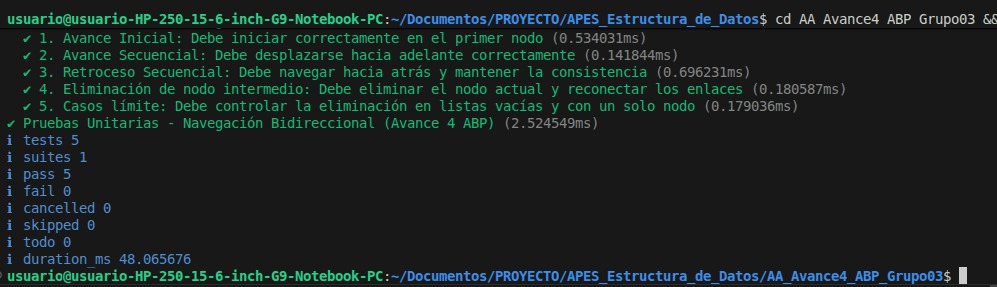
\includegraphics[width=0.6\textwidth]{Figuras/consola_pruebas.png}
    \caption{Resultado de \texttt{node -{}-test} tests/navegacion.test.js: 5 de 5 pruebas aprobadas.}
    \label{fig:consola}
\end{figure}


%%%%%%%%%%%%%%%%%%%%%%%%%%%%%%%%%%%%%%%%
\section{Conclusiones}
%%%%%%%%%%%%%%%%%%%%%%%%%%%%%%%%%%%%%%%%
% Responsable: Integrante 5. Dos o tres puntos cortos.

\begin{itemize}[leftmargin=*]
\item La lista doblemente enlazada permite navegar en ambas
direcciones mediante referencias al nodo anterior y siguiente,
facilitando el desplazamiento entre elementos.
\item Las cinco pruebas unitarias ejecutadas permitieron
verificar el correcto funcionamiento de la inicialización,
el avance, el retroceso, la eliminación de nodos y los
casos límite de la lista doblemente enlazada.
\item El uso de Git y GitHub permitió organizar el trabajo
colaborativo, integrar los aportes de los integrantes y
mantener un registro de los cambios realizados.
\end{itemize}


%%%%%%%%%%%%%%%%%%%%%%%%%%%%%%%%%%%%%%%%
\section{Declaración de ética e inteligencia artificial}
%%%%%%%%%%%%%%%%%%%%%%%%%%%%%%%%%%%%%%%%
% Responsable: Integrante 5. Cada integrante debe pasarle qué IA usó y sus prompts.

Para la organización y revisión del formato del presente
informe se contó con el apoyo de ChatGPT (OpenAI),
principalmente en aspectos relacionados con LaTeX.
Cada integrante es responsable de su aporte y de
verificar la información presentada.


%%%%%%%%%%%%%%%%%%%%%%%%%%%%%%%%%%%%%%%%
% Bibliografía: se genera sola desde Referencias.bib en formato APA 7
\nocite{*}            % Incluye todas las referencias del .bib aunque no se citen
\printbibliography

\end{document}
